\newpage
\section{Experiments}
\subsection{Setup and parameter selection}
The experiment uses one million 256-bit documents, top 100 results, a 32 GB decimal worker
budget, one CPU thread, and one query at a time on an Apple M5 Max with 128 GiB of physical
memory. A, B and C share the complete binary score and ID tie rule. Routing and the
Python-to-C++ call are included in retrieval time; document preparation and query encoding
are excluded. Fresh processes build and warm each configuration before measurement.

The controlled corpus retains the earlier random document signs after hash verification.
Fresh queries use seed 20260912: 32 for tuning and 64 for evaluation in each of the fixed and
changing-position cases. Both have twelve strong coordinates. Parameters are frozen before
the evaluation; no query is removed because its match count or timing is inconvenient.

The declared family contains no-routing search, direct prefix widths 4,8,10,11,12,13,14, and
IVF cluster counts 256 and 4096. Probe counts come from tuning-only recall cutoffs and the
fixed-prefix calculation. Every method receives every available layout and probe count.
B additionally varies leaf size, including 288 and 320 from the derivation and a scan-sized
leaf. C varies key width and uses coordinates after the routing prefix. Both local searches
have unlimited work budgets in this comparison.

There are 130 fixed-position and 299 changing-position tuning settings. Each has two timing
repetitions. Each chosen setting is evaluated in three process blocks with two repetitions
per query. Worker order is shuffled. Memory and power settings are recorded; unchanged
settings do not prove constant CPU frequency. Process memory includes construction, which
is stricter than checking only the stored index.

\begin{figure}[H]\centering
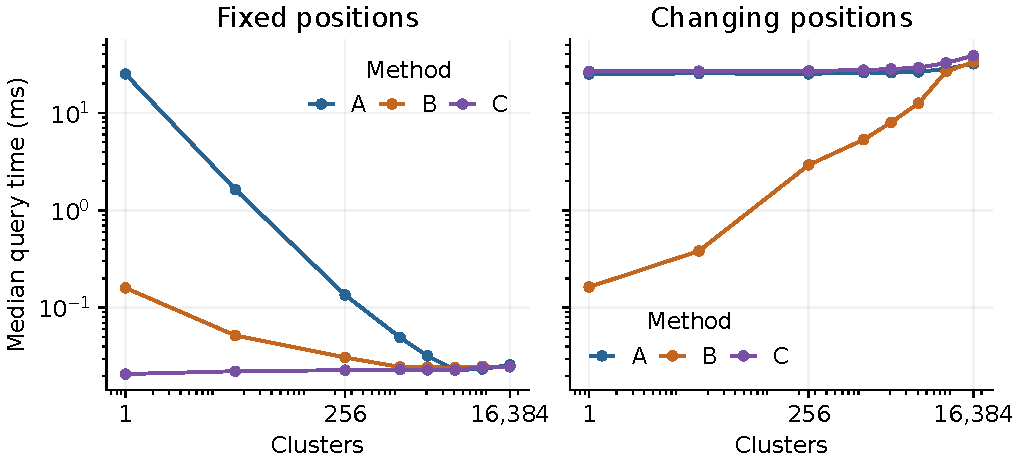
\includegraphics[width=\linewidth]{figures/tuning-clusters.pdf}
\caption{The fastest eligible \emph{tuning} setting at each cluster count, after allowing each
method its local settings and the available routers. These curves expose the cluster-size
choice. They do not select new parameters from evaluation data or interpolate untested optima.}
\label{fig:cluster-curves}
\end{figure}

The measured selection uses each method's fastest tuning setting whose lower recall estimate
meets 99\%. A separate selection minimizes the calibrated time model over eligible settings.
Analytic work estimates are used only for supported uniform-sign paths; other cases use
explicitly labeled tuning work estimates. Routing cost and recall eligibility remain empirical
for arbitrary layouts. Both selections are evaluated when they differ.

\newpage
\subsection{Checking and revising the model}
The first model correctly counted the applicable search work but assigned overly simple
prices to it. Across tuning cases, 380 fixed-position and 253 changing-position count predictions
matched native counters exactly. Other observations remained in the study, outside those
particular formulas. However, some initial B/C time estimates differed by up to 69\%.

One B example, a global index with leaf size 4096, was predicted at 0.265 ms but measured at
0.600 ms. A zero leaf word starts no scoring; a nonempty word begins a short run of row
accesses. The first model did not distinguish this access pattern from scoring consecutive
rows. Under uniformly distributed survivors, the expected nonempty leaf-word count is
\begin{equation}
 V_{\rm nonempty}\approx V_l\left[1-\left(1-\frac{F_B}{wV_l}\right)^w\right].
 \label{eq:nonempty}
\end{equation}
For C, an empty directory lookup does less work than a successful lookup that starts a
document range. A uniform-occupancy approximation estimates successful posting starts as
\begin{equation}
 H_{\rm hit}\approx H\frac{U}{C_{\rm stored}2^h}.
 \label{eq:posting-hits}
\end{equation}
Here $U$ is the occupied-entry count and $C_{\rm stored}$ the number of stored cluster
directories. Query-selected cells may not be representative, so this remains an approximation.

The revised model adds a fitted cost for each of these terms; the failed first fit remains
saved. Using the revised coefficients in the earlier depth guide gives approximately 13.5
for fixed positions and 11.5 for changing positions. Only depths 0--12 satisfy this experiment's
strong-coordinate assumption.
The added nonempty-word term is nonlinear, so every valid integer depth is checked under
the revised model. Both conditions select twelve cuts for the global path.

\begin{figure}[H]\centering
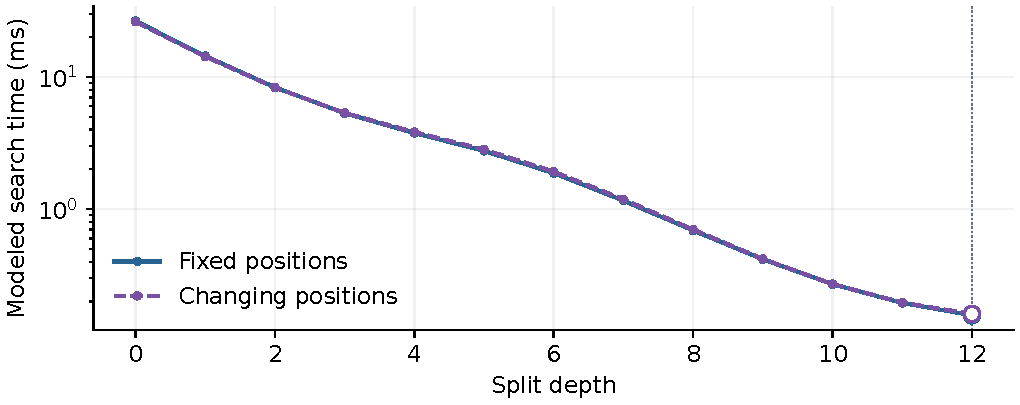
\includegraphics[width=.87\linewidth]{figures/global-branch-depth.pdf}
\caption{The revised global B model evaluated at all thirteen valid integer depths, including
zero. The curve describes the constructed single-path case and calibrated costs. It does
not assume that arbitrary real queries follow one branch.}
\end{figure}

The revision reduced the changing-position B maximum tuning error from 43.2\% to 19.2\%.
Some C tuning errors still reach 39\% in the changing case and 52\% in the fixed case.
The 20\% acceptance threshold was not changed. These remaining failures limit the model's
range; a small predicted difference is insufficient to establish a winner. Final evaluation
checks the selected settings without refitting their coefficients.

\newpage
\subsection{Controlled comparisons}
\begin{table}[H]\centering\small
\caption{Frozen tuning choices on separate queries. Peak memory includes construction.}
\begin{tabular}{@{}lllrrrrr@{}}
\toprule
Condition & Method & Route $C/P$ & $L$ & $h$ & Recall (\%) & ms & Peak MB \\
\midrule
Fixed & A & Prefix 4,096/1 & -- & -- & 100.00 & 0.0227 & 189.5 \\
Fixed & B & Prefix 4,096/1 & $N$ & -- & 100.00 & 0.0234 & 225.4 \\
Fixed & C & Global 1/1 & -- & 12 & 100.00 & 0.0207 & 136.7 \\
Changing & A & Global 1/1 & -- & -- & 100.00 & 25.0578 & 154.0 \\
Changing & B & Global 1/1 & 288 & -- & 100.00 & 0.1649 & 185.8 \\
Changing & C & Global 1/1 & -- & 8 & 100.00 & 26.7614 & 136.8 \\
\bottomrule
\end{tabular}

\end{table}
The settings in the table were selected using tuning queries, then measured on 64 separate
queries. Their peak process memory is well below 32 GB. The fixed-position scan chooses
4096 direct prefix clusters and one probe. Backward walk chooses a global 12-bit key; both
select the same ideal group. B's selected large leaf performs no splits in this case.

When important coordinates change, the selected bitplane setting instead uses one global
cluster and leaf size 288. Its query-dependent coordinate order removes most document scores
without requiring a fixed key to capture the important positions. A and C also had access
to all declared cluster layouts; neither was forced to use the same router as B.

\begin{table}[H]\centering\small
\caption{Paired time ratios. A ratio above one favors the method in the denominator.}
\begin{tabular}{@{}llrrl@{}}
\toprule
Condition & Time ratio & Estimate & 95\% interval & Faster \\
\midrule
Fixed & A/B & 0.971 & [0.932, 1.029] & -- \\
Fixed & A/C & 1.099 & [1.070, 1.127] & C \\
Fixed & B/C & 1.131 & [1.094, 1.158] & C \\
Changing & A/B & 151.980 & [150.917, 152.810] & B \\
Changing & A/C & 0.936 & [0.906, 0.942] & A \\
Changing & B/C & 0.00616 & [0.00595, 0.00623] & B \\
\bottomrule
\end{tabular}

\end{table}
Each interval resamples queries and whole process blocks with paired method observations.
Repeated timings are not additional independent queries. A speed advantage is supported
only when both choices meet the recall and memory requirements and the entire 95\% ratio
interval exceeds one. The fixed-position C advantage concerns the implemented routing and
lookup organization; it does not establish an asymptotic advantage over direct prefix scanning.

\begin{table}[H]\centering\small
\caption{Frozen model choices: predicted and measured median retrieval times.}
\begin{tabular}{@{}llrrrrl@{}}
\toprule
Condition & Method & Predicted ms & Measured ms & Error (\%) & Recall (\%) & Same setting \\
\midrule
Fixed & A & 0.0245 & 0.0223 & +9.7 & 100.00 & Yes \\
Fixed & B & 0.0226 & 0.0240 & -6.0 & 100.00 & No \\
Fixed & C & 0.0198 & 0.0210 & -5.6 & 100.00 & Yes \\
Changing & A & 26.2454 & 26.3998 & -0.6 & 100.00 & Yes \\
Changing & B & 0.1630 & 0.1661 & -1.9 & 100.00 & Yes \\
Changing & C & 27.8237 & 26.7609 & +4.0 & 100.00 & No \\
\bottomrule
\end{tabular}

\end{table}
All six model-selected settings reached 100\% recall and their median-time predictions were
within 10\% of the new measurements. Two selected parameter records differ from the
measured-tuning choice: fixed B uses leaf 320 instead of a scan-sized leaf, and changing C
uses one key bit instead of eight. The former still performs no split on these opened
clusters. This agreement is evidence for the selected operating points, not a guarantee
that every setting in the larger grid is predicted within 20\%.

\newpage
\subsection{Real-data replication}
The real-data control repeats the earlier frozen choices on the same 200 MS MARCO/Nomic
evaluation queries~\cite{msmarco,nomic}. It is a replication, not a new-query generalization
test. The original tuning covered 6821 settings; this run preserves each method's chosen
layout and local settings, then repeats them in three new process blocks.

\begin{table}[H]\centering\small
\caption{Replication of the frozen real-data choices at the 99\% target.}
\begin{tabular}{@{}lllrrrrr@{}}
\toprule
Condition & Method & Route $C/P$ & $L$ & $h$ & Recall (\%) & ms & Peak MB \\
\midrule
Real data & A & IVF 4,096/1,536 & -- & -- & 99.25 & 10.1050 & 183.4 \\
Real data & B & IVF 4,096/1,536 & 1024 & -- & 99.25 & 10.4267 & 220.5 \\
Real data & C & IVF 4,096/1,536 & -- & 4 & 99.25 & 12.5883 & 154.9 \\
\bottomrule
\end{tabular}

\end{table}
\begin{table}[H]\centering\small
\caption{Mean work per query. Timing repetitions are not extra count samples.}
\begin{tabular}{@{}llrrrr@{}}
\toprule
Condition & Method & Rows scored & Split words & Leaf words & Key lookups \\
\midrule
Fixed & A & 243.3 & 0.0 & 0.0 & 0.0 \\
Fixed & B & 243.3 & 0.0 & 4.2 & 0.0 \\
Fixed & C & 243.3 & 0.0 & 0.0 & 1.0 \\
Changing & A & 1,000,000.0 & 0.0 & 0.0 & 0.0 \\
Changing & B & 244.7 & 187,744.1 & 15,869.1 & 0.0 \\
Changing & C & 808,626.4 & 0.0 & 0.0 & 207.0 \\
Real data & A & 375,897.1 & 0.0 & 0.0 & 0.0 \\
Real data & B & 375,897.1 & 0.0 & 6,622.3 & 0.0 \\
Real data & C & 375,897.1 & 0.0 & 0.0 & 24,576.0 \\
\bottomrule
\end{tabular}

\end{table}

A was fastest in this replication. The paired 95\% intervals for A/B and A/C were
0.963--0.974 and 0.787--0.818, respectively; both exclude one.

The work counts explain why an algorithm's name is insufficient to interpret its timing.
In the real 99\% comparison, all three methods score the same selected documents. B's large
leaves avoid splitting but still require mask enumeration. C enumerates the four-bit keys
inside the selected clusters. Neither alternative saves full document scores at that
operating point, so their extra work cannot be interpreted as successful pruning.

The controlled case asks a different question. With changing important coordinates, B's
full-width mask work is worthwhile because it avoids nearly all row scores. With fixed
important coordinates, A and C both obtain a small group directly. The parameter choices,
native counters and complete retrieval timings must be read together.

\subsection{Code and evidence}
\begin{center}\small
\begin{tabularx}{\linewidth}{@{}lY@{}}\toprule
Paper component & Repository entry point\\\midrule
Three search implementations & \path{cpp/index.cpp}, \path{cpp/key_index.cpp}, \path{cpp/score.hpp}\\
Distribution and depth formulas & \path{experiments/optima_model.py}\\
Preparation, tuning, evaluation & \path{experiments/optima_study.py}\\
Initial/revised time predictions & \path{experiments/optima_predictions.py}\\
Native conditional count checks & \path{experiments/check_controlled.py}\\
All inputs, failures and observations & \path{results/optima-2026-09-12/}\\\bottomrule
\end{tabularx}\normalsize
\end{center}
The source README gives the exact commands. Raw cases are archived with file hashes; the
first failed model remains in \path{predictions-v1/}. The plots and tables are generated
from saved results. Rebuilding the PDF does not rerun the experiment.
